\section{Obtaining frequency from sound}
The current method of controlling the car is based on sound input.
When the game is running, voice input is continually recorded and analysed, in order to detect the pitch of the sound input, so that the direction in which to move the car can be decided.
The current method of analysing this is by using Fast Fourier's Transformation (FFT) and subsequently choosing the loudest frequency.

In this section we will briefly explain what sound is, in order to understand how to obtain certain characteristics of sound.
Based on this knowledge we will argue why it is difficult to obtain frequency from a sound input, especially sound input with human voice.
The technicalities in the section are based on the work of \citet*{music-and-computers}.

\subsection{Characteristics of sound}
Sound is a physical phenomenon which acts like a wave and therefore has the same characteristics as a wave.
So basically sound is a movement of air and the way we perceive sound is an interpretation of these movements.

Simply speaking, the volume (or loudness) of a sound, is the amplitude of the sound wave.
The pitch of a sound, how high/low we perceive it, is the frequency of the sound wave.
These two characteristics are independent, meaning that two sound waves with same frequency, but different amplitudes, will sound like the same pitch, but one being louder than the other.
An example can be seen in \cref{fig:samepitchdiffamp}.

\begin{figure}[h]
\centering
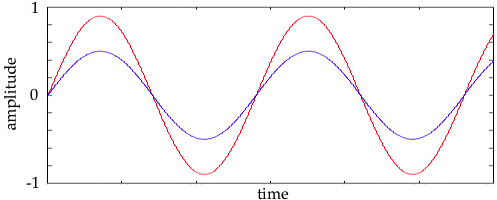
\includegraphics[width=.80\textwidth]{sprint1/samepitchdiffamp}
\caption{Two sound waves (represented as sine functions) with same frequency, but different amplitude.}
\label{fig:samepitchdiffamp}
\end{figure}

There is also a third characteristic, which is more abstract and not directly a physical attribute, namely, timbre.
Timbre is a composition of different sound waves (spectra), which makes up a specific sound (again, this is perceptual) and envelope (transients), which describe the different stages of a sound.
\subsection{Obtaining frequency}\label{obtaining_frequency}
The frequency of a sound can be obtained from a sound input interpreted as a wave (sine function).
However, some sounds are simpler than others in their composition of waves.
These simpler sounds could be considered ''cleaner'' than others, meaning they consist of only a single or very few waves, where it is easy to identify a primary amplitude and frequency.

Human speech, among other sounds, consists of multiple sound waves, each with varying amplitude and frequency.
In this case, it may be difficult to identify a single wave as the most important, and choose its frequency as the main frequency.
A comparison between frequency spectra can be seen in \cref{fig:frequency_spectra}.

\begin{figure}[h]
\centering
\begin{subfigure}[t]{.45\textwidth}
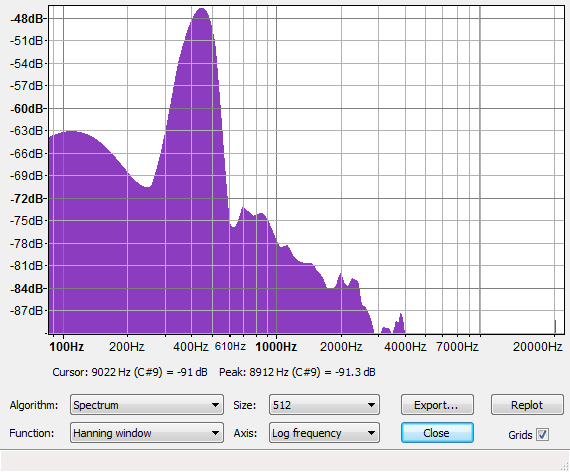
\includegraphics[width=\textwidth]{sprint1/spectrum_tonegenerator}
\caption{Frequency spectrum for a 440 Hz generated tone}
\end{subfigure}
\begin{subfigure}[t]{.45\textwidth}
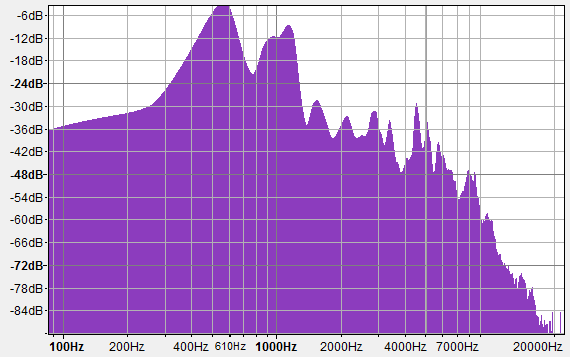
\includegraphics[width=\textwidth]{sprint1/spectrum_highpitchvoice}
\caption{Frequency spectrum for human voice input (in an attempt to reach 1200Hz)}
\label{fig:humanvoice_spectra}
\end{subfigure}
\caption{Frequency analysis in Audacity}
\label{fig:frequency_spectra}
\end{figure}

\subsection{Using FFT}
Fast Fouriers Transform (FFT) is a method of extracting the smaller components of a sound input.
As mentioned previously, a sound is a composition of several sound waves with each their own frequency and amplitude.
Therefore the result of the FFT on a sound input, is the existing frequencies and their amplitudes.
The result is called a frequency spectrum and can be seen in \cref{fig:frequency_spectra}.

\subsubsection{Cars and FFT}
In Cars, part of the method of extracting a frequency from the sound recording, is by using FFT.
How and why exactly the frequency spectrum is used for extracting a single frequency was not properly documented in the Cars report, it is only certain that the result from the FFT and the following manipulation leads to the loudest frequency value.
This value is then used in comparison with the calibrated low and high threshold values, to determine in which direction to move the car.

This poses several problems.
Firstly, human speech is complex and contains many different individual sound waves.
What sounds to us like a high pitch voice, can easily peak at a much lower frequency, as higher amplitude low frequency sounds will not always sound as loud as lower amplitude high frequency sounds.
This is due to our perception of sound.
An example of this can be seen in \cref{fig:humanvoice_spectra}, where in an attempt to hit a high frequency of approximately 1200 Hz, the highest peak was actually at approximately 600 Hz.

Another problem is the method of grouping together frequencies linearly in the FFT method.
Our hearing is logarithmic, meaning that a slight change in frequency is much more apparent to our perception at lower frequencies, than at higher frequencies.
When analysing the input, frequencies are not registered as their exact frequency, but are grouped together in ranges, linearly.
This means that lower frequencies that are very different in regards to pitch may be grouped together.
This impacts the result of the analysis, where one group of frequencies will have a higher amplitude, without it being the one we thought was the most apparent to our perception.
